The frontend design of the Blockchain Transaction Information Visualization System emphasizes user-centric interaction and information clarity through a thoughtfully structured interface. The design approach balances sophisticated functionality with intuitive user experience, making complex blockchain data accessible to users of varying technical backgrounds. 
\begin{figure}[h]
    \centering
    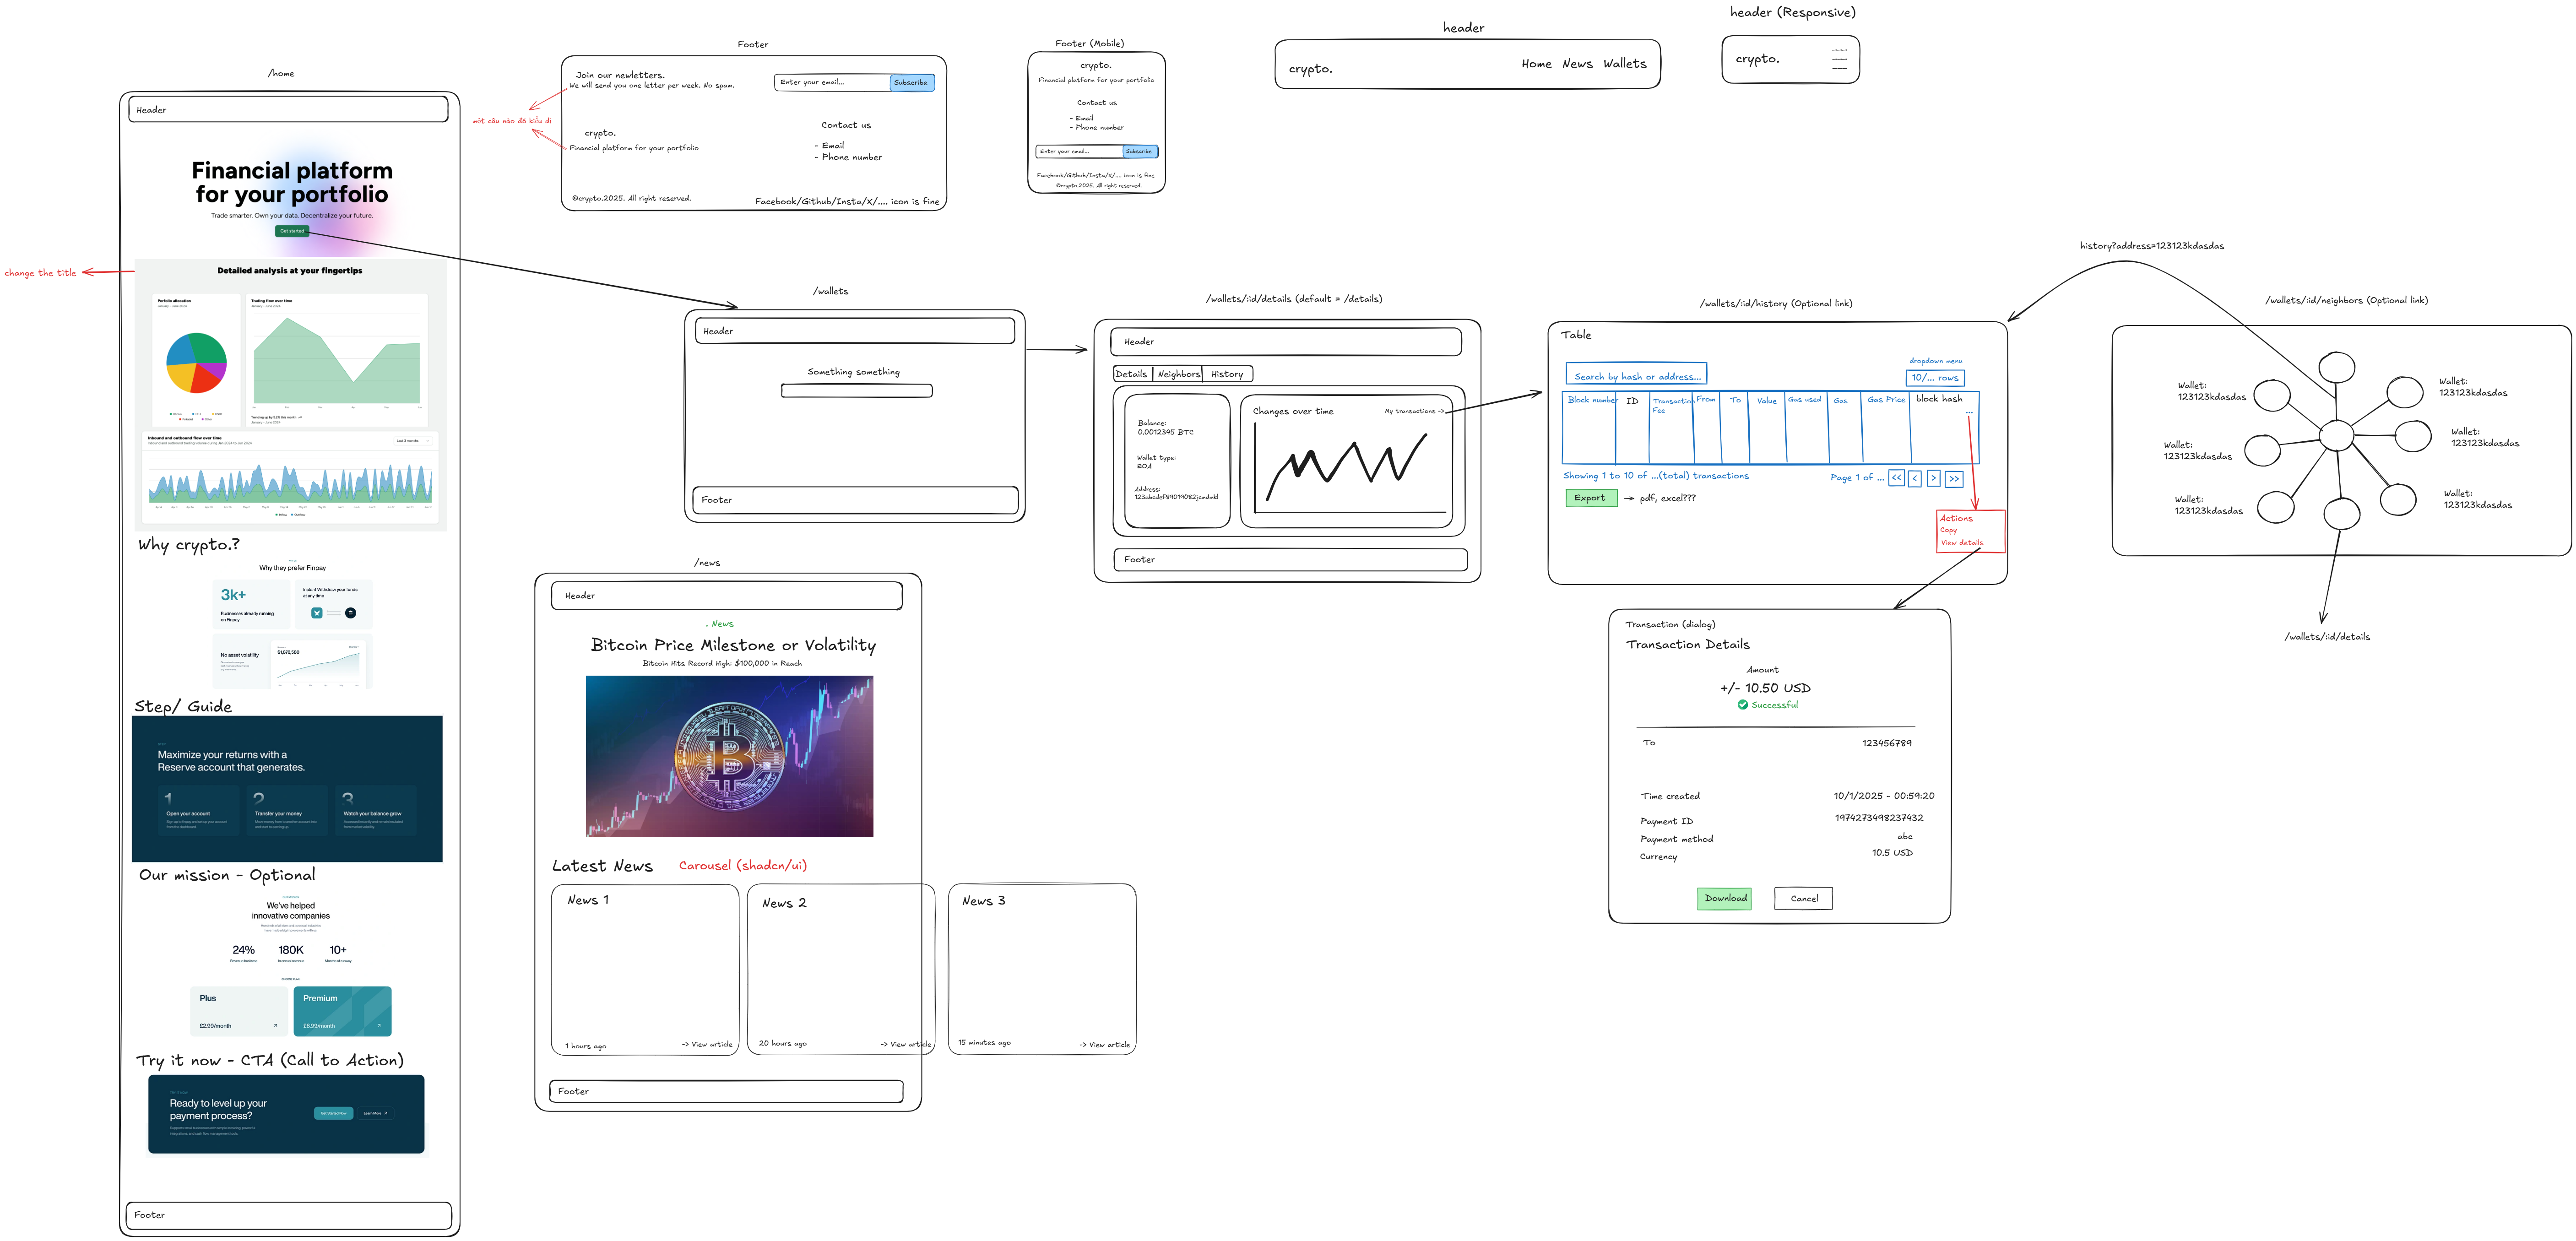
\includegraphics[width= 1\textwidth,  keepaspectratio]{root/image.png}
    \caption{Front-end prototype. \href{https://excalidraw.com/\#room=9d4fa2b42691ec469547,47-HCI7BFUW576wjGYaIXw}{Demo link}}
    \label{fig:prototype}
\end{figure}
\section{Design Principles}
The design principles for our platform (Figure \ref{fig:prototype}) establish a clean and efficient user experience through thoughtful minimalism and clear hierarchy. By removing unnecessary elements, the interface allows users to focus on essential features while maintaining intuitive navigation. The platform's responsive design ensures seamless adaptation across devices, from mobile phones to desktop computers, while maintaining visual consistency through unified elements like rounded corners and strategic whitespace. Professional typography and careful spacing work together to enhance readability and reinforce brand identity. These integrated design choices create a cohesive, trustworthy financial interface that balances functionality with refined aesthetics, delivering a professional experience that meets users' needs across all touchpoints.
\section{Prototype Explanation}
\subsection{Header and Footer}
 Header and footer will be implemented globally across our platform to  provide essential navigation, communication channels, and legal information in an organized and accessible manner, supporting the platform's overall user experience goals.
\begin{figure}[h]
    \centering
    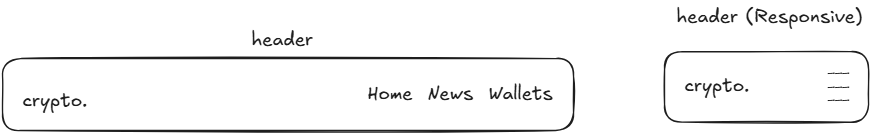
\includegraphics[width= 0.9\textwidth,  keepaspectratio]{root/header.png}
     \caption{Header}
    \label{fig:header}
\end{figure}
\paragraph{} The desktop header (Figure \ref{fig:header}) has a clean, minimalist design with "crypto." aligned to the left as the logo/brand name, and a horizontal navigation menu to the right containing three links: "Home," "News," and "Wallets." The responsive mobile version maintains the "crypto." branding on the left but replaces the navigation menu with a hamburger menu icon ($\equiv$) on the right, which is a common pattern for collapsing navigation options on smaller screens. Both headers appear to use a simple black and white color scheme with rounded rectangle borders containing the elements.
  \begin{figure}[h]
    \centering
    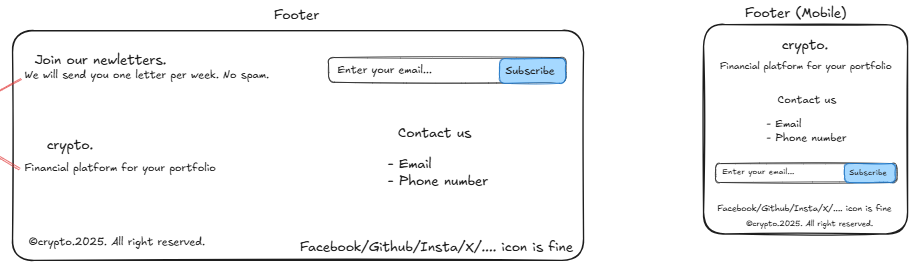
\includegraphics[width= 0.9\textwidth, keepaspectratio]{root/footer.png}
     \caption{Footer}
    \label{fig:footer}
\end{figure}
\paragraph{}The footer in Figure \ref{fig:footer} design demonstrates a thoughtful approach to responsive web design with desktop and mobile versions. The desktop layout spreads content horizontally, featuring a newsletter subscription section with a clear "no spam" promise, email input field, and a subscribe button. The company branding "crypto." appears with its descriptive tagline "Financial platform for your portfolio" alongside contact options for email and phone. Social media integration is indicated for platforms like Facebook, GitHub, Instagram, and X, though currently shown as text placeholders. The mobile version adapts this content into a vertical stack while maintaining all key elements, optimizing space usage for smaller screens. Both versions include the copyright notice "crypto.2025. All right reserved." and share a consistent minimalist black and white color scheme, ensuring a cohesive user experience across devices.
\subsection{Homepage}
\begin{figure}[h]
    \centering
     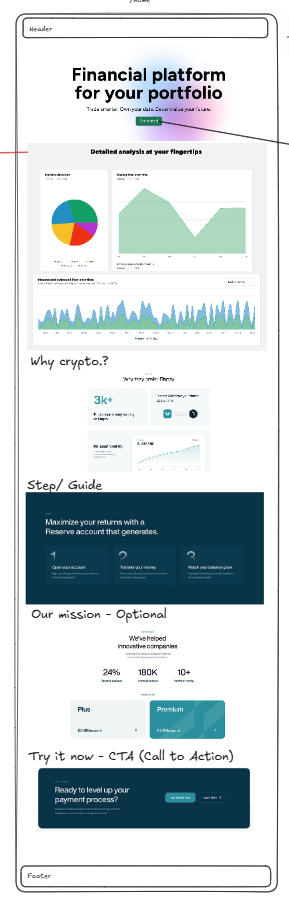
\includegraphics[width= \textwidth, height=0.595\textheight, keepaspectratio]{root/homepage.png}
    \caption{Homepage}
    \label{fig:homepage}
\end{figure}
\paragraph{}Our homepage (Figure \ref{fig:homepage}) embodies a user-centric design philosophy, emphasizing minimalism and intuitive navigation. The layout is strategically segmented into distinct functional sections that serve dual purposes: showcasing our system's core capabilities while providing a clear onboarding path for new users. Each section is thoughtfully crafted to maintain visual hierarchy and guide visitors through a seamless exploration of our platform.
  \begin{figure}[h]
    \centering
    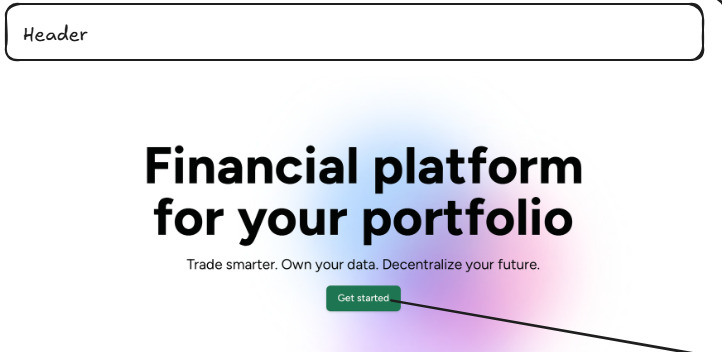
\includegraphics[width= 0.8\textwidth, keepaspectratio]{root/hero.png}
     \caption{Hero section}
    \label{fig:hero}
\end{figure}
\paragraph{}The homepage prototype begins with a clean and modern header section ( see Figure \ref{fig:hero}). Below it, the hero section showcases a bold headline "Financial platform for your portfolio" against a crisp white background. This background is artfully decorated with three floating spherical elements in different colors, creating a subtle but dynamic visual interest. The spheres appear to be gently moving in the space, adding a touch of playfulness to the professional design. A prominent green call-to-action button stands out beneath the headline, inviting users to begin their journey with the platform. The entire hero section effectively combines simplicity with visual appeal, immediately communicating the platform's purpose while maintaining an engaging and modern aesthetic.
 \begin{figure}[h]
    \centering
    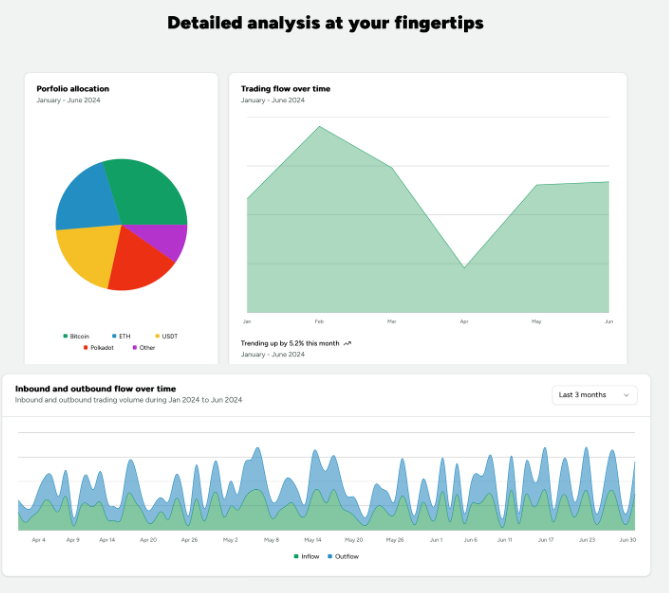
\includegraphics[width= 0.9\textwidth, 
    height=0.6\textheight, keepaspectratio]{root/analysis.png}
     \caption{Visualizations}
    \label{fig:analysis}
\end{figure}

\paragraph{}Next part of the homepage is the dashboard section (Figure \ref{fig:analysis}). This section showcases three distinct visualization types - a pie chart representing portfolio allocation, an area chart displaying trading flow trends, and a detailed inbound/outbound flow graph - providing potential users with a comprehensive preview of the platform's analytical capabilities. These interactive visualizations serve as a powerful demonstration of the system's ability to transform complex blockchain transaction data into clear, actionable insights, allowing visitors to immediately grasp the platform's value proposition. The visualizations employ a minimalist design approach with a professional color scheme of soft greens and blues, complemented by strategic accent colors. The layout features a clean grid system with balanced spacing and subtle shadows, while clear sans-serif typography maintains information hierarchy. Interactive elements like time period selectors and smooth transitions enhance user engagement, all while maintaining a sophisticated yet approachable aesthetic that makes complex financial data easily digestible.
 \begin{figure}[h]
    \centering
    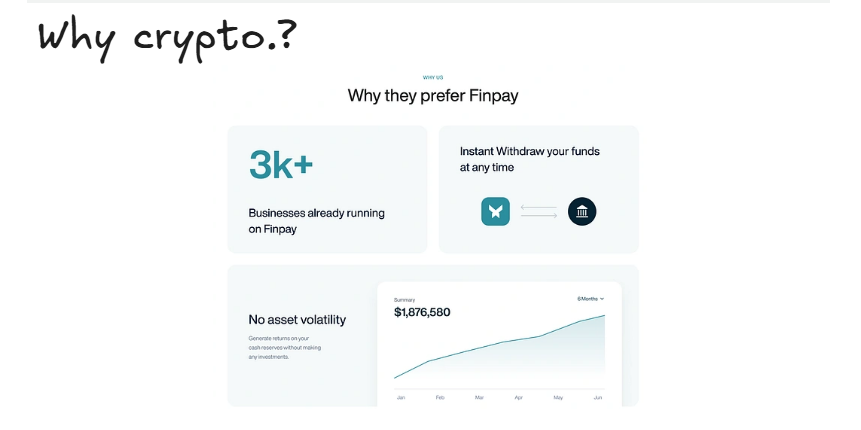
\includegraphics[width= 0.9\textwidth, keepaspectratio]{root/why.png}
     \caption{Why Choose Us page layout}
    \label{fig:Why choose us}
\end{figure}
\paragraph{}In this "Why Choose Us" section (see Figure \ref{fig:Why choose us}), we address typical concerns about cryptocurrency trading while highlighting our key strengths through a streamlined, intuitive interface. Our clean, minimalist design approach makes complex trading concepts more approachable, while reinforcing user confidence through visual clarity. Features are displayed in harmoniously styled cards, creating a cohesive visual narrative that emphasizes both professionalism and ease of use. This carefully structured presentation helps demystify cryptocurrency trading for newcomers while offering the depth that experienced traders expect, with each benefit clearly articulated to demonstrate our platform's value.
\begin{figure}[h]
    \centering
    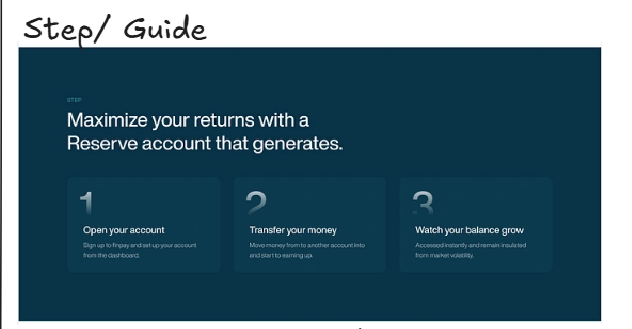
\includegraphics[width= 0.9\textwidth]{root/step.png}
     \caption{Guide for users to start}
    \label{fig:step}
\end{figure}
\paragraph{}The homepage continues with tutorial sections (Figure \ref{fig:step}), which showcase a meticulously designed onboarding section for cryptocurrency trading, featuring a streamlined three-step process presented in a sophisticated dark-themed interface. The intuitive design hierarchy, led by a compelling and appropriate headline, guides users through essential stages: wallet creation, account funding, and trading initiation. Each step is thoughtfully presented with consistent visual elements, including numbered cards, descriptive text, and thematic icons in an engaging green accent color. The clean layout and clear information architecture effectively communicate both simplicity and professionalism, while the "Learn more" links provide depth as well as clear tutorial without overwhelming new users. This design aims to balance the complexity of cryptocurrency trading with an approachable user experience, making it particularly effective for both newcomers and experienced traders looking for a straightforward platform.

\paragraph{} The "Our Mission" section (refer to \ref{fig:option}) presents a thoughtfully designed pricing and impact showcase that effectively combines social proof with subscription options. The layout employs a clean, hierarchical structure beginning with impressive statistics, which immediately establishes credibility and scale of impact. Below these metrics, the section transitions smoothly into a dual-tier pricing structure featuring "Plus" and "Premium" plans, priced at \pounds 2.99 and \pounds 5.99 per month respectively. The design utilizes a subtle yet effective color contrast, with the Premium tier highlighted in a professional teal color against the Plus tier's neutral background, subtly guiding users toward the higher-value option. The pricing cards maintain a clean, minimalist approach with clear monthly pricing and directional arrows, making the selection process straightforward and uncluttered. This section successfully balances social proof with commercial offerings, while the "Optional" notation suggests flexibility in implementation, allowing for strategic placement within the broader platform design.
\begin{figure}[h]
    \centering
    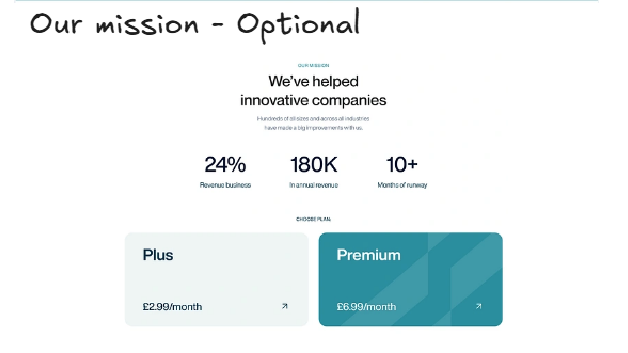
\includegraphics[width= 0.9\textwidth]{root/option.png}
     \caption{Pricing plan and impact showcase}
    \label{fig:option}
\end{figure}
\paragraph{} The Call-to-Action (CTA) section, see Figure \ref{fig:cta}, displays a sophisticated and compelling design approach within a deep navy-colored banner that draws immediate attention. The section will lead with an engaging question, for example "Ready to level up your payment process?", which creates a direct connection with potential users while highlighting the platform's core value proposition. The layout will employ a clean, horizontal structure with a supporting subheading that emphasizes business benefits and management tools. Two distinct action buttons - "Get Started Now" and "Learn More" - provide clear pathways for users at different stages of the decision-making process, with the primary CTA featuring a contrasting color to drive conversions. The dark background paired with light text creates strong visual contrast, ensuring readability while maintaining a professional, fintech-appropriate aesthetic. This CTA section effectively balances urgency with professionalism, using strategic spacing and typography to create a clean, uncluttered call to action that encourages user engagement without appearing overly aggressive.
\begin{figure}[h]
    \centering
    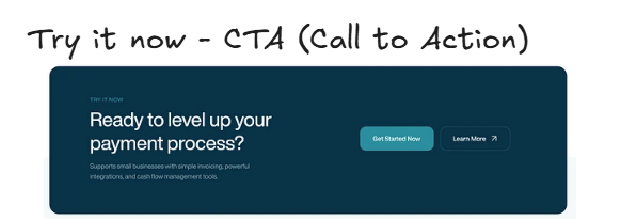
\includegraphics[width= 0.9\textwidth]{root/cta.png}
     \caption{Call to action}
    \label{fig:cta}
\end{figure}
\paragraph{}This compelling Call-to-Action section serves as the homepage's final touchpoint, strategically positioned immediately above the footer. Acting as a powerful closing statement, it provides a clear pathway for user conversion while maintaining the sleek, professional aesthetic established throughout the page.

\subsection{News page}
\begin{figure}[h]
    \centering
    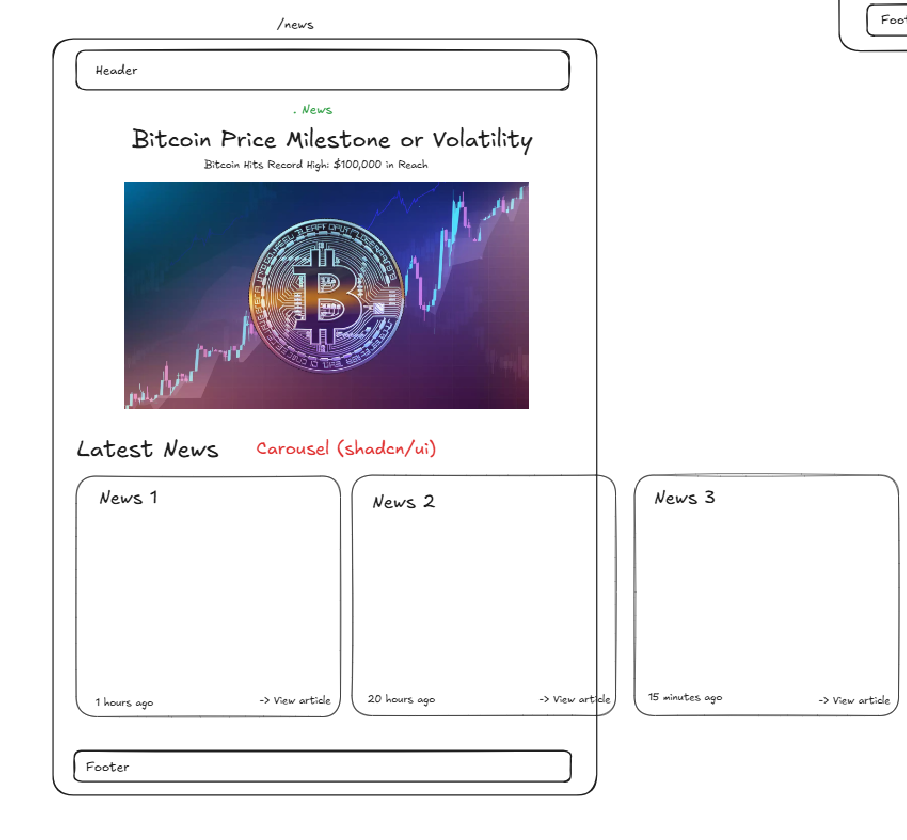
\includegraphics[width= 0.8\textwidth, height=0.6\textheight]{root/news.png}
     \caption{News page}
    \label{fig:news}
\end{figure}
\paragraph{}This news page design showcases a thoughtfully structured layout that effectively delivers cryptocurrency news content through a clear visual hierarchy. The page opens with a prominent header containing navigation links, leading into a featured story section that commands attention .Below, a "Latest News" carousel implemented using shadcn/ui components displays three news cards, each featuring timestamps and "View article" links, creating a dynamic flow of information. The design maintains professional credibility while ensuring easy navigation, with clear timestamps, providing content recency, and consistent spacing throughout the layout enhancing readability.
\subsection{Wallets page}
\paragraph{}When users navigate to the Wallets page (Figure \ref{fig:search}), they will land on a screen featuring a search bar. By entering a wallet address into this search bar, users can retrieve and view the detailed information associated with that specific wallet.
\begin{figure}[h]
    \centering
    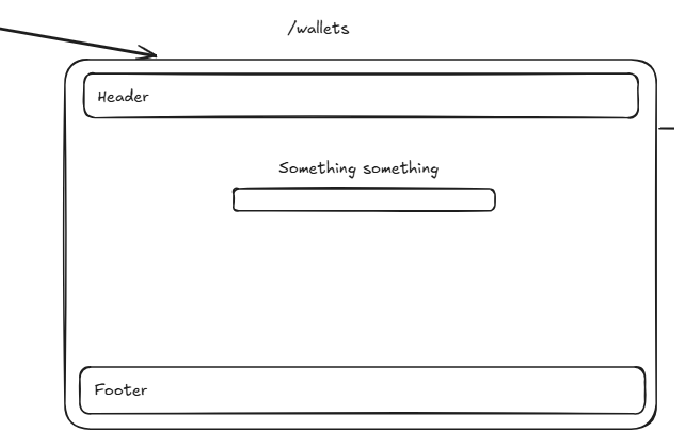
\includegraphics[width= 0.6\textwidth, keepaspectratio]{root/search.png}
     \caption{Search page}
    \label{fig:search}
\end{figure}
\paragraph{}After entering a correct wallet address, users will be navigated to wallet details page (Figure \ref{fig:Wallet_Detail}), accessed via the route /wallets/:id/details. The design of this page employs a traditional web application structure with header and footer elements framing the main content area. The interface features a prominent three-tab navigation system (Details, Neighbors, History), with Details serving as the default view. The main content is thoughtfully divided into two primary panels: the left panel displays essential wallet information including the BTC balance (0.0012345 BTC), wallet type (EOA), and a truncated wallet address, while the right panel showcases a dynamic line graph titled "Changes over time" that visualizes transaction or value history with notable fluctuations.
\begin{figure}[h]
    \centering
    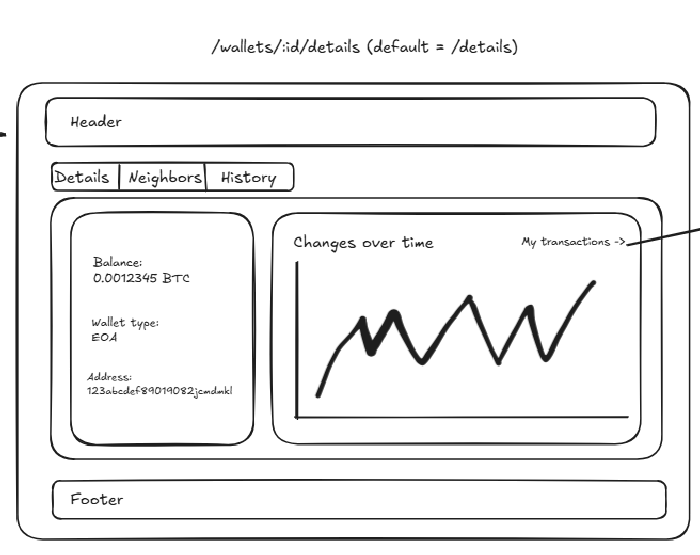
\includegraphics[width= 0.6\textwidth, keepaspectratio]{root/wallet_wallets.png}
     \caption{Wallet Details}
    \label{fig:Wallet_Detail}
\end{figure}
\paragraph{} The Wallet Pages include ``My Transactions'' and ``History'' options in the navigation bar (Figure \ref{fig:Wallet_Detail}). Clicking either of these options takes the user to a comprehensive view of the transaction history, refer to Figure \ref{fig:history}, for the selected wallet.

To enhance usability, the transaction history table incorporates several practical features:

\begin{itemize}
  \item \textbf{Search bar:} Allows filtering transactions by hash or address
  \item \textbf{Pagination:} Enables navigating through transaction records page by page
  \item \textbf{Export options:} Supports exporting transaction data in PDF or Excel file formats
\end{itemize}

Selecting an individual transaction from the table opens a detailed transaction dialog window. This dialog provides in-depth information about the selected transaction, such as:

\begin{itemize}
  \item Precise date and time of the transaction
  \item Associated payment IDs
  \item Exact transaction amounts
  \item Clear success/failure status indicators
\end{itemize}

This thoughtfully designed combination of a comprehensive transaction history table and detailed drill-down dialogs empowers users to easily navigate, analyze, and manage their wallet's transaction records.
\begin{figure}[h!]
    \centering
    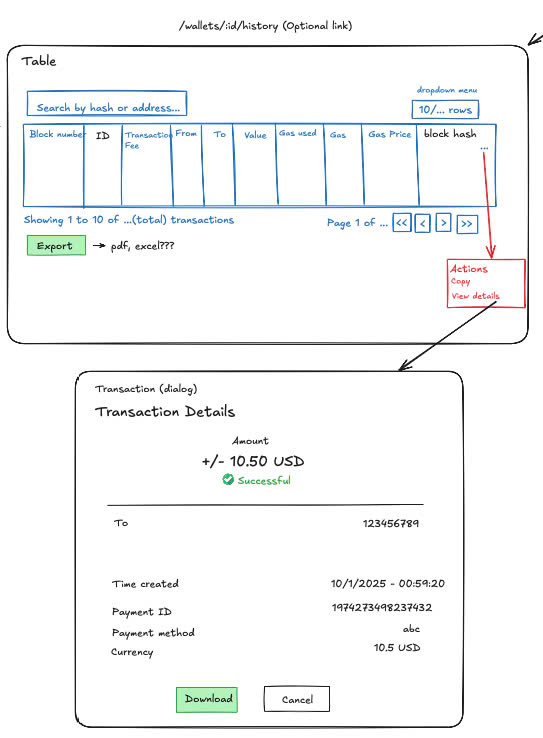
\includegraphics[width= 0.5\textwidth, height=0.73\textheight, keepaspectratio]{figures/test.jpg}
     \caption{Wallet Transaction History}
    \label{fig:history}
\end{figure}

\paragraph{} The /wallets/id/neighbors page (Figure \ref{fig:graph}) displays an interactive network visualization that shows how different wallets are connected through transactions. In this graph, each point (or node) represents a unique wallet address.  This interactive visualization allows users to explore and analyze transactions by clicking on nodes or edges to view specific details such as transaction amounts, timestamps, and associated metadata (transaction details in a table on the /wallets/id/history), see Figure \ref{fig:history}. Each wallet node is labeled with an unique wallet address.

\paragraph{}But why we need to add this graph visualization to our platform? Incorporating this visualization into our blockchain visualization platform offers several benefits. It enables users to easily explore and trace the flow of funds, potentially detecting suspicious activities or anomalies indicative of fraud or money laundering. The graph provides insights into wallet connectivity and relationships, identifying central wallets acting as transaction hubs and discovering closely connected wallet communities. Also, the user-friendly visual representation enhances transparency and accessibility, making it easier for users to understand and trace fund movements without delving into complex raw transaction data.

\begin{figure}[H]
    \centering
    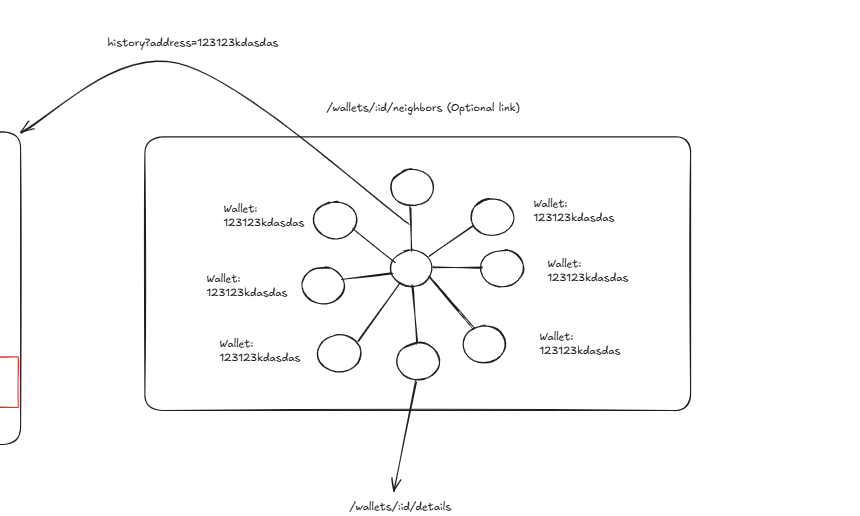
\includegraphics[width= 0.7\textwidth]{root/graph.png}
     \caption{Transactions Depicted in Graph Format}
    \label{fig:graph}
\end{figure}





 
 
